\documentclass[11pt,a4paper,oneside]{book}

% Packages
\usepackage{caption}
  \captionsetup{font=footnotesize}
\usepackage{fullpage}
\usepackage{geometry}
  \geometry{verbose,tmargin=2cm,bmargin=2.5cm,lmargin=2.5cm,rmargin=2.5cm,footskip=1.5cm}
\usepackage{graphicx}
\usepackage[colorlinks=true, linkcolor=blue, citecolor=blue]{hyperref}
\usepackage{mathtools}
\usepackage[round]{natbib}
  \bibliographystyle{plainnat}
\usepackage{setspace}
  \onehalfspacing

% User-defined commands
\newcommand{\latex}{\LaTeX\xspace} % latex symbol

% Path for graphs
\graphicspath{{images/}}


% ===== TITLE =====================================================================================
\title{From Crosses to Micro Foundations:\\
The Stepping Stone from Monetary Economics in the IS-LM Model to the New-Keynesian paradigm}

\author{
  Jane Doe (coordinator)
  \and
  John Doe
  \and
  Ana Smith
}
% =================================================================================================

\begin{document}
\frontmatter
\maketitle

% ===== ABOUT THIS NOTES ==========================================================================
\chapter{About these notes}
The main objective of these notes is to create a reference document that can be useful to all students who want to review bridge the gap between the IS-LM model and the New Keynesian paradigm.

As a chapter author, your job is \textbf{NOT} to put together a lot of information that is difficult and tiring to read. Keep always in mind that measuring the quality of your chapter by the lines or pages written is like measuring aircraft building progress by weight.\footnote{This is an adaptation of a code from Bill Gates that says "Measuring programming progress by lines of code is like measuring aircraft building progress by weight".} Your job is to facilitate learning and understanding. To explain something to somebody else requires that you deeply \textbf{understand} what you are explaining. Hence, your first job is to understand the concepts you need to explain. Then you need to reflect in which is the best way to present those concepts to facilitate learning. Lastly, you have to make sure that the document produced actually accomplishes the purpose for which it is created.

The main sources of information you have are the class slides and what is discussed during the lectures. However, your chapter should not be a transcript of what was explained during each session. You need to create a narrative that connects the concepts covered and helps the reader understand these concepts and the context in which they are relevant. Look into the textbooks, recommended readings, references, etc. and enhance the information covered in the class.

This work is licensed under a \href{http://creativecommons.org/licenses/by-nc/4.0/}{Creative Commons Attribution-NonCommercial 4.0 International License}.

\tableofcontents
\listoffigures
\listoftables
% =================================================================================================

\mainmatter

% ===== TEMPLATE CHAPTER ==========================================================================
\chapter{Template chapter}
\label{ch:template_chapter}
In this chapter you can find a short guideline on how to properly design your chapter. The information here should be almost enough to write your chapter. You should only need external sources to clarify questions you might have. In other words, \textbf{try to keep your document as simple as possible}.

Please use British English.

The best online reference for \latex is the \href{https://en.wikibooks.org/wiki/LaTeX}{Wikibook on \latex}. Moreover, a Google search tends to solve more of the problems one might face.

% ----- DOCUMENT STRUCTURE ------------------------------------------------------------------------
\section{This is a section}
\label{sec:document_structure}
Organising the information you want to present on your chapter is as important as the information itself. When your write your chapter, you can use sections, subsections, and even \textit{subsubsections}. Make sure not to over do it.

For more information on document structure see \href{https://en.wikibooks.org/wiki/LaTeX/Document_Structure}{this} section the \latex Wikibook.
\section{This is another section}
\subsection{This is a subsection}
\subsubsection{And this is a subsubsection}
% -------------------------------------------------------------------------------------------------

% ----- FLOATS ------------------------------------------------------------------------------------
\section{How to present a graph or table}
\label{sec:floats}
To use a graphs we need to create a float-figure like this one:
% ----- BEGIN GRAPH
\begin{figure}[h!]
  \centering
    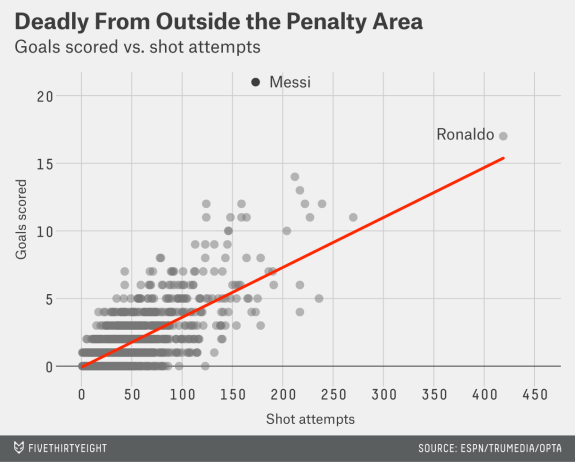
\includegraphics[width=0.25\textwidth]{example}
    \caption{The capiton of each graph should contain a brief description of what appears in the graphs (if the table in the graph is not enough), all the relevant information regarding the type of data displayed, its source, and (if need it) the author of the graph.}
    \label{fig:messi_vs_ronaldo}
\end{figure}
% ----- END GRAPH

Note that all files that contain graphs are saved in the folder \textit{images}. The preferred format for a graph is EPS.

A Table can be created easily by:
% ----- BEGIN TABLE
\begin{table}[h!]
  \centering
    \begin{tabular}{| l c r |}
    \hline
    1 & 2 & 3 \\
    4 & 5 & 6 \\
    7 & 8 & 9 \\
    \hline
    \end{tabular}
  \caption{A simple table.}
  \label{tab:simple_table}
\end{table}
% ----- END TABLE

Creating rich tables can be cumbersome. There are online tools that can help, like \href{https://www.tablesgenerator.com/}{tablesgenerator.com}.

For more information on floats see \href{https://en.wikibooks.org/wiki/LaTeX/Floats,_Figures_and_Captions}{this} section the \latex Wikibook.
% -------------------------------------------------------------------------------------------------

% ----- CITATION ----------------------------------------------------------------------------------
\section{How to cite books, articles, and other parts of the same document}
\label{sec:citations}
The management of a bibliography in \latex is extremely important. If properly done, it can save lots of time and effort. The bibliography in this document is organised as follows. There is a file, named "monetary.bib" in that contains all the information on the items cited. Strictly speaking this file is a BiBTeX file. In order to cite an item, the first thing you need to do is to add that item to the BibTeX file. To do so, you can either use a bibliography manager, such as \href{http://www.jabref.org/}{JabRef} or you can directly edit the BiBTeX file. I strongly recommend you use the first option if you are new to \latex.

Then you need to cite the item within the document. Here you have a citation of an academic article: \citet*{Cooley_Hansen_1989}. Books are cited exactly in the same way within the document: \citet*{Blanchard_2017}. For more information on bibliography management see \href{https://en.wikibooks.org/wiki/LaTeX/Bibliography_Management}{this} section the \latex Wikibook.

To reference another part of the document is very easy, it only requires creating a label and a reference: see section \ref{sec:citations}. You also use cross-references to refer to figures and tables, like Figure \ref{fig:messi_vs_ronaldo} or Table \ref{tab:simple_table}. For more information on labels and cross-referencing see \href{https://en.wikibooks.org/wiki/LaTeX/Labels_and_Cross-referencing}{this} section the \latex Wikibook.
% -------------------------------------------------------------------------------------------------

% ----- MATH --------------------------------------------------------------------------------------
\section{How to present equations}
\label{sec:math}
In \latex it is very easy to work with equations and mathematical expresions. For example one can easily insert mathematical expressions in the text by writting $ a = \frac{b}{c} \times \beta $. Equations can also be inserted by:
\begin{equation}
  f(x)=(x+a)(x+b)
  \label{eq:function}
\end{equation}
Equations can also be referenced, like Equation \ref{eq:function}. For more information on mathematics in \latex see \href{https://en.wikibooks.org/wiki/LaTeX/Mathematics}{this} section the \latex Wikibook.


% -------------------------------------------------------------------------------------------------
% =================================================================================================

% ...

% \appendix
% \chapter{First Appendix}

\backmatter
\bibliography{monetary.bib}


\end{document}
